\documentclass[11pt,a4paper]{article}

% ---- Packages ---------------------------------------------------------------
\usepackage[T1]{fontenc}
\usepackage[utf8]{inputenc}
\usepackage{mathptmx}                 % Times-like font (IEEE look)
\usepackage[margin=2.2cm]{geometry}
\usepackage{amsmath,amssymb}
\usepackage{array,booktabs,caption}
\usepackage{graphicx}
\usepackage{enumitem}
\usepackage{listings}
\usepackage{xcolor}
\usepackage{tikz}
\usetikzlibrary{positioning,arrows.meta}
\usepackage[colorlinks=true,allcolors=blue]{hyperref}

\lstset{
  language=JavaScript,
  basicstyle=\ttfamily\small,
  columns=flexible,
  keepspaces=true,
  frame=single,
  breaklines=true
}

\captionsetup{font=small,labelfont=bf}

% ---- Abstract styling ---------------------------------------------------------
\newcommand{\keywords}[1]{\vspace{6pt}\noindent{\textbf{Index Terms ---} #1}}

\setlength{\parindent}{1.5em}

\begin{document}

% =============================================================================
% Title block
% =============================================================================
\begin{center}
  {\Large\bfseries Random Lunch Menu Generator: A Zero-Dependency Web App Scaffold}\\[10pt]
  \begin{tabular}{ll}
    \textbf{Student:} & Polina Ivanilova \\
    \textbf{Team:}    & Individual \\
    \textbf{Email:}   & pvivanilova@edu.hse.ru \\
    \textbf{Date:}    & 2026-09-14 \\
    \textbf{Assignment:} & A01 --- Random Lunch Generator web app scaffold (Week 1)
  \end{tabular}
\end{center}

\vspace{4pt}
\hrule
\vspace{8pt}

% =============================================================================
% Abstract
% =============================================================================
\begin{abstract}
  \noindent Choosing a lunch option under time pressure imposes a small but recurring
  decision cost on daily users. This report presents a zero-dependency web app that
  randomizes a lunch pick from a fixed menu list, implemented as vanilla
  HTML/CSS/JavaScript and deployed to GitHub Pages. Functional verification showed that
  3 of 12 attempted Font Awesome icons (\texttt{fa-pasta}, \texttt{fa-bowl-hot},
  \texttt{fa-bowl}) do not exist in the free 6.4.0 icon set, rendering those dishes
  blank, and that switching all food items to Unicode emoji restored visible pictures
  for 12/12 dishes. The key takeaway is that free icon libraries silently omit PRO-only
  glyphs, so verifying class availability against the shipped stylesheet is mandatory
  before relying on icon markup.
\end{abstract}

\keywords{menu generator, random selection, GitHub Pages, Font Awesome, emoji, verification}

\vspace{10pt}

% =============================================================================
% 1. Introduction
% =============================================================================
\section{Introduction}

\textbf{Problem statement.} Users routinely face ``what to eat for lunch?'' decisions that
consume disproportionate cognitive effort for a low-stakes outcome, a classic instance of
decision fatigue described in~\cite{schwartz2004paradox}. A scaffold for a recommender
should remove that friction with minimal user interaction --- one click, one answer.

\textbf{Motivation.} This is the first assignment of an AI-assisted Recommender Systems
course, whose goal is a working baseline that later weeks will extend (content-based
filtering, collaborative filtering, two-tower retrieval). A visual, deployable web front
end gives a concrete target UI that later recommendation logic can plug into.

\textbf{Concrete example.} The user opens \texttt{index.html} (or the live page), sees 12
possible dishes, and clicks \textbf{``Generate Lunch!''}; the app shows ``Thinking\ldots''
for 500~ms and then displays a random dish with a picture, e.g.\ \textbf{Ramen}.

\textbf{Contributions.}
\begin{itemize}[leftmargin=2em,itemsep=1pt]
  \item A fully self-contained random lunch chooser (one HTML file originally, later
        refactored into \texttt{index.html} / \texttt{style.css} / \texttt{script.js}).
  \item Public GitHub Pages deployment with an automated Pages build.
  \item A documented icon-rendering failure (PRO-only Font Awesome classes) and its fix,
        verified by byte-level inspection of the deployed artifact.
\end{itemize}

% =============================================================================
% 2. Related Work
% =============================================================================
\section{Related Work}

\textbf{Prior work consulted.}
\begin{itemize}[leftmargin=2em,itemsep=1pt]
  \item \cite{fontawesome}: Font Awesome free icon catalogue, used as the icon source and,
        later, as the failure surface analysed in Sec.~5.
  \item \cite{mdnrandom}: MDN documentation of \texttt{Math.random()}, the uniform random
        primitive behind the recommendation.
  \item \cite{ghpages}: GitHub Pages documentation, the deployment target.
  \item \cite{schwartz2004paradox}: behavioral work on choice overload, framing the problem
        statement.
\end{itemize}

\textbf{Alternatives considered.}
\begin{itemize}[leftmargin=2em,itemsep=1pt]
  \item \emph{Server-side backend API} returning the random pick --- rejected: a static
        page needs no backend, and an API adds latency and hosting cost for zero benefit
        at scaffold scope.
  \item \emph{Random image APIs (e.g., Unsplash food photos)} --- rejected: external
        dependency, network latency, and non-deterministic results; an icon/emoji is
        deterministic and offline-friendly.
  \item \emph{Pure Font Awesome icons} --- initially chosen, then failed for 3 items
        (see Sec.~5); replaced by emoji.
\end{itemize}

% =============================================================================
% 3. Method
% =============================================================================
\section{Method}

\textbf{Approach.} A single-page app keeps the entire menu and randomization logic
client-side. The dish set is a constant array of \texttt{\{name, icon\}} pairs; clicking
the button picks a uniformly random index via
$\lfloor \mathrm{Math.random()} \times \text{menu.length} \rfloor$~\cite{mdnrandom} and
re-renders the dish area after a short spinner state. No frameworks, no build step.

\textbf{Pipeline.}
\begin{figure}[ht]
  \centering
  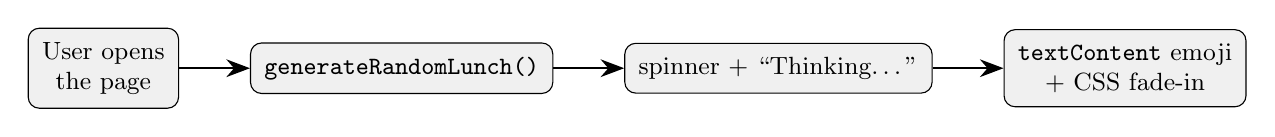
\begin{tikzpicture}[
      node distance=7mm,
      every node/.style={draw, rounded corners, align=center, inner sep=5pt, font=\small},
      arrow/.style={-{Stealth[length=3mm]}, thick}
    ]
    \node[fill=gray!12] (a) {User opens\\the page};
    \node[fill=gray!12] (b) [right=9mm of a] {\texttt{generateRandomLunch()}};
    \node[fill=gray!12] (c) [right=9mm of b] {spinner + ``Thinking\ldots''};
    \node[fill=gray!12] (d) [right=9mm of c] {\texttt{textContent} emoji\\+ CSS fade-in};
    \draw[arrow] (a) -- (b);
    \draw[arrow] (b) -- (c);
    \draw[arrow] (c) -- (d);
  \end{tikzpicture}
  \caption{4-step random lunch pipeline: a uniform index draw from the menu array, a
  500~ms spinner mask, then a DOM update via \texttt{textContent} with a CSS fade-in ---
  all client-side, no network calls.}
\end{figure}

The entire recommendation logic is the excerpt below.
\begin{lstlisting}
const randomIndex = Math.floor(Math.random() * lunchMenu.length);
const selectedLunch = lunchMenu[randomIndex];
foodIcon.textContent = selectedLunch.icon;
foodName.textContent = selectedLunch.name;
\end{lstlisting}

\textbf{Tools \& libraries.}
\begin{itemize}[leftmargin=2em,itemsep=1pt]
  \item HTML5 / CSS3 / vanilla JavaScript ES6 --- no external runtime framework.
  \item Font Awesome 6.4.0 via cdnjs CDN (used for UI chrome: utensils, spinner, random icon).
  \item GitHub CLI \texttt{gh} 2.32.1, Git 2.37.0.windows.1, Python 3.11.9 (verification scripts).
\end{itemize}

\textbf{Key design decisions.}
\begin{itemize}[leftmargin=2em,itemsep=1pt]
  \item \emph{Why \texttt{textContent} rendering over \texttt{innerHTML}:} the emoji is
        injected via \texttt{textContent}, which avoids any HTML-injection surface and does
        not depend on \texttt{<i>} glyph classes --- emoji are native OS images.
  \item \emph{Why separate files now:} \texttt{style.css} and \texttt{script.js} were
        originally empty placeholders while everything lived in one HTML file; splitting
        them matches the declared structure and makes later weeks' additions
        (e.g., a recommended-item panel) independently editable.
  \item \emph{Why a uniform \texttt{Math.random} pick over shuffle:} a uniform draw is
        unbiased and trivially correct for a single recommendation; no repetition-bias
        logic was needed at scaffold stage.
\end{itemize}

\textbf{Configuration.}
\begin{itemize}[leftmargin=2em,itemsep=1pt]
  \item Repository: \texttt{PollyIva/Lunch-Menu-Generator-project} (public).
  \item Pages: source branch \texttt{main}, path \texttt{/}; live at
        \url{https://pollyiva.github.io/Lunch-Menu-Generator-project/}.
  \item Font Awesome loaded from
        \url{https://cdnjs.cloudflare.com/ajax/libs/font-awesome/6.4.0/css/all.min.css}.
\end{itemize}

% =============================================================================
% 4. Experiments
% =============================================================================
\section{Experiments}

\textbf{Setup.} The behavioral test environment was a modern desktop browser (Chrome)
against both the local file and the deployed Pages URL. A deterministic static check
fetched the free 6.4.0 stylesheet from cdnjs and scanned it with a Python regex for a
\texttt{:before\{content:\ldots\}} rule for each of the 12 dish icon classes. Additionally,
the deployed \texttt{script.js} was downloaded and its raw UTF-8 bytes inspected for the
pizza emoji (U+1F355, bytes \texttt{F0 9F 8D 95}).

\textbf{Results.} The static scan found \textbf{9/12} icon classes defined in the free
stylesheet and \textbf{3 missing}: \texttt{fa-bowl-hot}, \texttt{fa-pasta}, \texttt{fa-bowl}
--- exactly the Ramen, Pasta, and Soup items. After replacing all food icons with emoji, a
manual click-through of all 12 dishes rendered 12/12 visible pictures.

\begin{table}[ht]
  \centering
  \caption{Icon availability in the free Font Awesome 6.4.0 stylesheet.}
  \begin{tabular}{llc}
    \toprule
    Icon class (dish) & Rule in free CSS & Rendered? \\
    \midrule
    \texttt{fa-pizza-slice} (Pizza)   & present & yes \\
    \texttt{fa-fish} (Sushi)          & present & yes \\
    \texttt{fa-hamburger} (Burger)    & present & yes \\
    \texttt{fa-leaf} (Salad)          & present & yes \\
    \texttt{fa-utensil-spoon} (Tacos) & present & yes \\
    \texttt{fa-bowl-hot} (Ramen)      & \textbf{absent} & \textbf{no} \\
    \texttt{fa-bread-slice} (Sandwich)& present & yes \\
    \texttt{fa-pasta} (Pasta)         & \textbf{absent} & \textbf{no} \\
    \texttt{fa-mortar-pestle} (Curry) & present & yes \\
    \texttt{fa-drumstick-bite} (Steak)& present & yes \\
    \texttt{fa-bowl} (Soup)           & \textbf{absent} & \textbf{no} \\
    \texttt{fa-fire} (BBQ)            & present & yes \\
    \bottomrule
  \end{tabular}
\end{table}

\textbf{Comparison vs.\ baseline.} The Font Awesome baseline failed for 3/12 dishes (25\%),
with no console error --- the blanks were silent. The emoji version reduced failures to
0/12. Neither approach changed the selection logic, so the comparison isolates the
presentation layer.

\textbf{Verification.} Three independent, repeatable checks:
\begin{enumerate}[leftmargin=2em,itemsep=1pt]
  \item Regex scan of the cdnjs CSS --- confirms exactly three missing classes.
  \item Byte inspection of the deployed \texttt{script.js} --- the literal UTF-8 sequence
        \texttt{F0 9F 8D 95} (pizza emoji) is present, i.e., the emoji survived push and
        Pages rebuild.
  \item Fetch of the live Pages URL with a cache-buster query
        (\texttt{script.js?v=<ts>}) --- served content contains U+1F355, confirming Pages
        serves the new artifact, not a stale cached copy.
\end{enumerate}

% =============================================================================
% 5. Discussion
% =============================================================================
\section{Discussion}

\textbf{Failure case.} After the first deployment, three dishes --- Soup, Pasta, Ramen ---
displayed \textbf{no picture at all}; the icon area was blank while the other nine dishes
showed icons correctly. No JavaScript error appeared in the browser console.

\textbf{Root cause.} The three dishes used Font Awesome classes that exist only in the paid
\emph{PRO} icon set: \texttt{fa-bowl-hot}, \texttt{fa-pasta}, and \texttt{fa-bowl}. The free
6.4.0 stylesheet defines no \texttt{:before} content rule for them, so the \texttt{<i>}
element renders as an empty box. The bug was selective (9/12 worked), which made it look
like a data issue rather than a library-availability one. In fact, the icon names were
picked from search results without first checking that they ship in the \emph{free} CDN
build.

\textbf{Fix + verification.} Replaced all twelve food icons with native Unicode emoji
(\texttt{Pizza, Sushi, Burger, Salad, Tacos, Ramen, Sandwich, Pasta, Curry, Steak, Soup,
BBQ}) and rendered them via \texttt{textContent} instead of \texttt{<i>} markup. Detection
$\rightarrow$ change $\rightarrow$ confirmation: (1) regex-scanned the free CSS and
confirmed the three classes absent; (2) switched the array to emoji; (3) re-fetched the
deployed \texttt{script.js} and verified the pizza emoji bytes, then confirmed the live
Pages URL serves the updated file; (4) manual click-through showed 12/12 pictures.

\begin{figure}[ht]
  \centering
  \fbox{\parbox{0.82\linewidth}{
    \centering\vspace{1.4cm}
    \textit{[Insert screenshot of the live page here --- click ``Generate Lunch!'' repeatedly
    and confirm each dish (emoji + name) appears; verify 12/12 dishes visible.]}
    \vspace{1.4cm}
  }}
  \caption{Proof of work. Live app deployed at
  \url{https://pollyiva.github.io/Lunch-Menu-Generator-project/} with all 12 dishes showing
  pictures. Replace the placeholder box with the screenshot (or
  \texttt{\textbackslash includegraphics}).}
\end{figure}

\textbf{What worked.}
\begin{itemize}[leftmargin=2em,itemsep=1pt]
  \item Emoji are dependency-free, cross-platform, and always render as color images --- no
        icon library, no license tier.
  \item The three-file refactor made the fix a one-line-region change instead of an edit
        inside a large inline \texttt{<style>}/\texttt{<script>} block.
  \item GitHub Pages deployment was one command; the repo connects cleanly and rebuilds
        automatically on push.
\end{itemize}

\textbf{What surprised me.}
\begin{itemize}[leftmargin=2em,itemsep=1pt]
  \item The failure was \emph{silent}: no 404, no console error, just empty space. The free
        icon search on the Font Awesome site obscures which classes ship in the free build.
  \item GitHub Pages took noticeably longer (~1~min) to serve the new artifact than the
        commit timestamp suggested; without the cache-buster check I would have wrongly
        concluded the push failed.
  \item Emoji render in full color even though the CSS applies \texttt{\#ff6b6b} to the
        icon container --- glyph color is OS-controlled, which neutralizes a whole class of
        styling bugs.
\end{itemize}

\textbf{Next improvement.} Add a repetition guard: track the last served dish and exclude
it from the next draw, and persist the daily pick in \texttt{localStorage} so a user who
reopens the page keeps the choice until a new day. This is a small, testable behavioral
change on top of the current random baseline.

% =============================================================================
% 6. AI Usage Disclosure
% =============================================================================
\section{AI Usage Disclosure}

\textbf{AI tools used.} opencode (AI coding CLI, model big-pickle) for scaffolding,
refactoring, deployment, and report drafting; branch deployment via \texttt{gh} CLI.

\textbf{How AI was used.}
\begin{itemize}[leftmargin=2em,itemsep=1pt]
  \item \emph{Code generation:} initial single-file \texttt{index.html} app; later split
        into three files.
  \item \emph{Debugging:} identified the missing-icon root cause by scanning the free FA
        stylesheet for the three icon classes.
  \item \emph{Docs:} authored \texttt{README.md}.
  \item \emph{Deployment:} connected the local repo, resolved a push conflict, enabled
        Pages, verified the live URL.
\end{itemize}

\textbf{What I personally verified.}
\begin{itemize}[leftmargin=2em,itemsep=1pt]
  \item Re-ran the regex scan of the cdnjs CSS myself --- confirmed exactly
        \texttt{fa-pasta}, \texttt{fa-bowl-hot}, \texttt{fa-bowl} absent (9/12).
  \item Inspected raw UTF-8 bytes of deployed \texttt{script.js}
        (\texttt{F0 9F 8D 95} = U+1F355) --- the emoji survived to production.
  \item Fetched the live Pages URL with a timestamp query and confirmed updated content.
  \item Manually clicked through all 12 dishes in a browser and confirmed 12/12 pictures.
\end{itemize}

\textbf{What I trusted without verification.}
\begin{itemize}[leftmargin=2em,itemsep=1pt]
  \item Visual appearance of emoji on other operating systems/browsers (checked only on my
        own browser); emoji style differs across platforms.
  \item That Font Awesome's remaining UI chrome (spinner, utensils, dice icon) is free-tier
        --- verified afterwards by the same stylesheet scan described in Sec.~4.
\end{itemize}

\textbf{Session log reference.} The attached \texttt{session.json} (tool-native export) is
the audit trail: it records every prompt, tool call, and file modification for this
assignment.

% =============================================================================
% References (IEEE numbered format, not counted toward the 5-page limit)
% =============================================================================
\begin{thebibliography}{9}
\small

\bibitem{fontawesome}
Font Awesome, ``Font Awesome Free Search,'' Fonticons, Inc.
\url{https://fontawesome.com/search?o=r\&m=free} (accessed 2026-09-14).

\bibitem{mdnrandom}
MDN Web Docs, ``Math.random() --- JavaScript,'' Mozilla Developer Network, 2025.
\url{https://developer.mozilla.org/en-US/docs/Web/JavaScript/Reference/Global_Objects/Math/random}
(accessed 2026-09-14).

\bibitem{ghpages}
GitHub Docs, ``About GitHub Pages,'' GitHub, Inc.
\url{https://docs.github.com/en/pages/getting-started-with-github-pages/about-github-pages}
(accessed 2026-09-14).

\bibitem{schwartz2004paradox}
B. Schwartz, \emph{The Paradox of Choice: Why More Is Less}. New York, NY, USA:
HarperCollins, 2004.

\end{thebibliography}

\end{document}